\documentclass[11pt]{article}

\usepackage[a4paper,margin=2.3cm]{geometry}
\usepackage{amsmath,amssymb}
\usepackage{tikz}
\usepackage{tikz-cd}
\usepackage{xcolor}
\usetikzlibrary{arrows.meta,positioning,calc,decorations.pathreplacing}

\title{\bfseries What is a trace map?\\[2pt]
\large A first--principles picture, in the language of categories}
\author{}
\date{}

\newcommand{\id}{\mathrm{id}}
\newcommand{\coev}{\eta}   % coevaluation
\newcommand{\ev}{\varepsilon} % evaluation
\newcommand{\Tr}{\operatorname{Tr}}
\newcommand{\tr}{\operatorname{tr}}
\definecolor{brick}{RGB}{0,90,160}
\definecolor{soft}{RGB}{245,247,250}

\begin{document}
\maketitle
\vspace{-1.2em}

\begin{center}
\emph{Goal: build the idea of a ``trace'' up from nothing, until the field trace
used in this project falls out as one special case.}
\end{center}

\hrule
\section*{1. The everyday trace}

For a square matrix, the trace is the sum of the diagonal entries.

\[
A=\begin{pmatrix}a&b\\ c&d\end{pmatrix},\qquad \tr A = a+d.
\]

One fact makes the trace special: \textbf{it does not depend on the basis you
chose.} If you change coordinates, $A$ becomes $PAP^{-1}$, but

\[
\tr(PAP^{-1})=\tr(A).
\]

So the trace is really attached to the \emph{linear map}, not to any matrix
picture of it. Anything that is independent of arbitrary choices is a hint that
a clean, choice--free (i.e.\ \emph{categorical}) description is hiding underneath.

\section*{2. What a category gives us}

A category is just \emph{objects} with \emph{arrows} (maps) between them that you
can compose. Our running example:

\begin{center}
\begin{tikzcd}[column sep=large]
\text{objects: vector spaces } U,V,W
  \arrow[r, no head, dashed]
& \text{arrows: linear maps } f\colon V\to W
\end{tikzcd}
\end{center}

To talk about trace we need two extra pieces of structure that vector spaces
have and that we can describe with arrows alone.

\medskip
\noindent\textbf{(a) A tensor product $\otimes$ and a unit object $I$.}
You can glue two spaces into $V\otimes W$, and there is a trivial one--dimensional
space $I=\Bbbk$ (the ground field) that acts as ``nothing added'':
$I\otimes V\cong V\cong V\otimes I$. A category with such a well--behaved
$\otimes$ and unit $I$ is called \emph{monoidal}.

\medskip
\noindent\textbf{(b) A dual $V^{*}$.}
Every finite--dimensional $V$ has a dual $V^{*}$ (the linear functionals on $V$),
and it comes with two canonical arrows:

\[
\begin{tikzcd}[row sep=tiny, column sep=huge]
I \arrow[r, "\coev"] & V\otimes V^{*}
& & V^{*}\otimes V \arrow[r, "\ev"] & I
\end{tikzcd}
\]

\begin{itemize}\setlength\itemsep{2pt}
\item \textbf{Evaluation} $\ev\colon V^{*}\otimes V\to I$ ``uses'' a functional
on a vector: $\ev(\phi\otimes v)=\phi(v)$.
\item \textbf{Coevaluation} $\coev\colon I\to V\otimes V^{*}$ is the basis--free
name for the identity matrix: $\coev(1)=\sum_i e_i\otimes e_i^{*}$.
\end{itemize}

An object with such a partner $V^{*}$, $\ev$, $\coev$ is called
\textbf{dualizable}. Finite--dimensional spaces are exactly the dualizable ones.

\section*{3. Trace as a single loop}

Here is the whole idea in one line. Take an endomorphism $f\colon V\to V$
(a map from a space to \emph{itself}). Feed the unit $I$ through this circuit:

\begin{center}
\begin{tikzcd}[column sep=2.4em, row sep=large]
I \arrow[r, "\coev"]
& V\otimes V^{*} \arrow[r, "f\,\otimes\,\id"]
& V\otimes V^{*} \arrow[r, "\text{swap}"]
& V^{*}\otimes V \arrow[r, "\ev"]
& I
\end{tikzcd}
\end{center}

The composite $I\to I$ is just multiplication by a number. \textbf{That number is
the trace of $f$}, written $\tr(f)$. No basis was ever mentioned.

\paragraph{The same thing as a picture (string diagram).}
Read time from bottom to top. A wire is the object $V$; the cap is $\coev$, the
cup is $\ev$; the box is $f$. Tracing = ``close the wire into a loop.''

\begin{center}
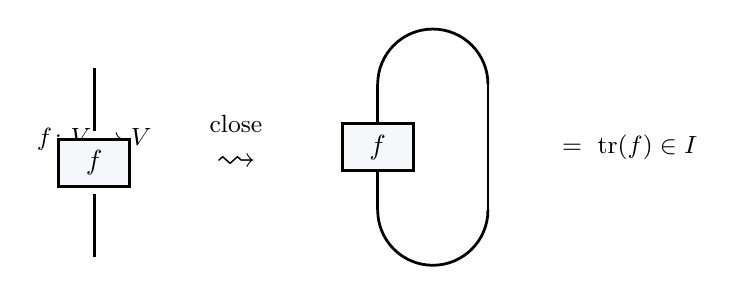
\begin{tikzpicture}[line width=1pt, scale=1.0]
% left diagram: f on a wire
\node at (-3.2,1.3) {\small $f\colon V\to V$};
\draw (-3.2,-0.2) -- (-3.2,0.6);
\draw (-3.2,1.4) -- (-3.2,2.2);
\node[draw, fill=soft, minimum width=0.9cm, minimum height=0.6cm] at (-3.2,1.0) {$f$};

% arrow
\node at (-1.4,1.0) {\Large $\rightsquigarrow$};
\node at (-1.4,1.5) {\small close};

% right diagram: closed loop = trace
\draw (0.4,0.4) -- (0.4,2.0);
\node[draw, fill=soft, minimum width=0.9cm, minimum height=0.6cm] at (0.4,1.2) {$f$};
% top cap (coev)
\draw (0.4,2.0) arc (180:0:0.7);
% right wire down
\draw (1.8,2.0) -- (1.8,0.4);
% bottom cup (ev)
\draw (0.4,0.4) arc (-180:0:0.7);
\node at (3.6,1.2) {\small $=\ \tr(f)\in I$};
\end{tikzpicture}
\end{center}

\noindent In coordinates this loop computes $\sum_i e_i^{*}\big(f(e_i)\big)
=\sum_i A_{ii}$, recovering ``sum of the diagonal.'' The categorical definition
just says the same thing without ever picking the $e_i$.

\paragraph{Why this is the ``right'' definition.}
It works in \emph{any} symmetric monoidal category with duals, not only vector
spaces, and it automatically obeys the properties we expect:
\[
\tr(g\circ f)=\tr(f\circ g),\qquad \tr(\id_V)=\dim V,\qquad
\tr(f\oplus g)=\tr f+\tr g .
\]
These are now theorems about the loop, provable by sliding boxes along the wire.

\section*{4. From ``trace of a map'' to ``trace map of a field''}

So far $\tr$ eats one endomorphism and returns a number. The \textbf{trace map}
of a field extension is what you get when you have a \emph{whole family} of
endomorphisms, one for every element of a bigger field.

\medskip
\noindent Let $K\subseteq L$ be a field extension. Viewed with $K$ as scalars,
$L$ is a $K$--vector space (finite--dimensional). Each $x\in L$ gives an
endomorphism
\[
m_x\colon L\to L,\qquad m_x(y)=x\cdot y \quad(\text{``multiply by }x\text{''}),
\]
which is $K$--linear. Now apply the loop of \S3 to every $m_x$ at once:

\begin{center}
\begin{tikzcd}[column sep=huge]
L \arrow[r, "x\ \mapsto\ m_x"] &
\{K\text{-endomorphisms of }L\} \arrow[r, "\tr\ (\text{\S3 loop})"] &
K
\end{tikzcd}
\end{center}

The composite $x\mapsto \tr(m_x)$ is the \textbf{field trace}
$\Tr_{L/K}\colon L\to K$. It is $K$--linear because $\tr$ is additive and
$m_{x+x'}=m_x+m_{x'}$.

\begin{center}
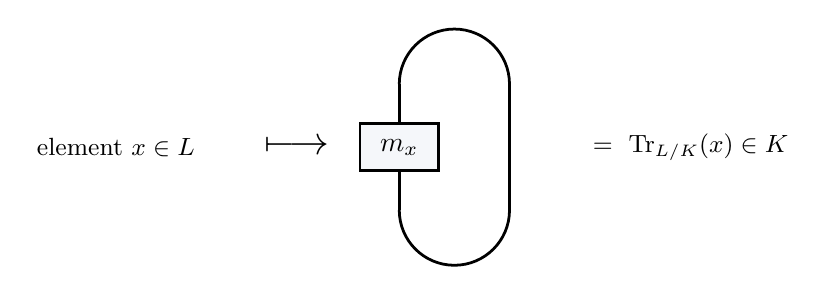
\begin{tikzpicture}[line width=1pt, scale=1.0]
\node at (0.0,1.2) {\small element $x\in L$};
\node at (0.0,0.9) {\small \phantom{x}};
\node at (2.3,1.2) {\Large $\longmapsto$};
% loop with m_x
\draw (3.6,0.4) -- (3.6,2.0);
\node[draw, fill=soft, minimum width=1.0cm, minimum height=0.6cm] at (3.6,1.2) {$m_x$};
\draw (3.6,2.0) arc (180:0:0.7);
\draw (5.0,2.0) -- (5.0,0.4);
\draw (3.6,0.4) arc (-180:0:0.7);
\node at (7.3,1.2) {\small $=\ \Tr_{L/K}(x)\in K$};
\end{tikzpicture}
\end{center}

\paragraph{One--line summary.}
\[
\boxed{\;\Tr_{L/K}(x)\ :=\ \tr\big(\,y\mapsto x\cdot y\,\big)\;}
\]
the field trace of $x$ is the categorical trace of ``multiply by $x$.''

\section*{5. What this project's trace is}

In this formalisation the ground field is $K=\mathbb{F}_2=\mathbb{Z}/2$ and $L$
is a finite field of characteristic $2$. Two facts pin everything down.

\medskip
\noindent\textbf{(i) Library trace $=$ categorical trace.}
Mathlib's \texttt{Algebra.trace K L} is defined as exactly the map of \S4:
\[
\texttt{Algebra.trace}\;K\;L\;(x)\ =\ \tr(m_x)\ =\ \Tr_{L/K}(x).
\]

\medskip
\noindent\textbf{(ii) Over $\mathbb{F}_2$ the loop becomes a Frobenius sum.}
For finite fields the trace has a closed form
(\texttt{FiniteField.algebraMap\_trace\_eq\_sum\_pow}):
\[
\Tr_{L/\mathbb{F}_2}(x)\ =\ \sum_{i=0}^{\,n-1} x^{2^{i}},
\qquad n=[L:\mathbb{F}_2].
\]
The right--hand side is precisely the project's own trace function
\texttt{Tr}\,/\,\texttt{truncTrace}. This equality is checked, \texttt{sorry}--free,
in \texttt{Equation1/TraceLibrary.lean}:

\begin{center}
\begin{tikzcd}[column sep=large, row sep=large]
x \arrow[r, "m_x"] \arrow[dr, "\displaystyle \sum_{i<n} x^{2^i}"'] &
\tr(m_x)=\texttt{Algebra.trace}\ \mathbb{F}_2\ L\ x \arrow[d, equal] \\
& \texttt{Tr}\ n\ x = \texttt{truncTrace}\ n\ x
\end{tikzcd}
\end{center}

\medskip
So the ``trace'' appearing throughout the equation--(1) development is not an
ad--hoc sum: it is the categorical loop of \S3 applied to the multiplication
endomorphisms of \S4, specialised to $\mathbb{F}_2$ where the loop unwinds into
the Frobenius sum $\sum_i x^{2^i}$.

\vfill
\hrule
\begin{center}\small
Diagrams: TikZ / tikz-cd. Rebuild with \texttt{tectonic TraceMap\_Categorically.tex}.
\end{center}

\end{document}
